\documentclass{article}
\usepackage{ctex}
\usepackage{amsmath}
\usepackage{graphicx}
\usepackage{wrapfig}
\usepackage{caption}
\usepackage[top=0.8in, bottom=0.8in,left=0.8in, right=0.8in]{geometry}
\usepackage{float} 
\usepackage{subfigure}
\usepackage{subcaption}
\usepackage{bm}
\usepackage{tikz}
\usetikzlibrary{arrows.meta}
% \xeCJKsetup{CJKmath=true} 
\begin{document}
\section*{van der Waals相互作用}
本题来研究\textit{van der Waals相互作用}.\par
% \subsection*{PART A.Van der Waals相互作用的产生与准备工作}
范德华相互作用是分子或原子间电偶(多)极矩之间的弱相互作用,包括:
\begin{itemize}
    \item[I]\textbf{偶极—偶极相互作用},又称\textit{Keesom force}:主要由自由旋转的极性分子之间的电偶极相互作用贡献,对所有旋转方向平均之后可以得到相互作用强度.%\begin{center}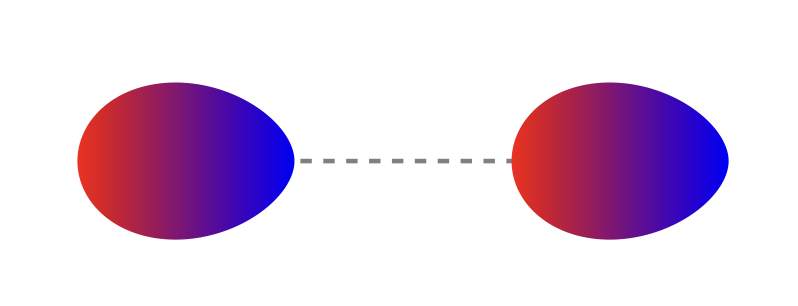
\includegraphics[scale=0.3]{img/0018.1.png}\end{center}
    \item[II]\textbf{偶极—感应偶极相互作用},又称\textit{Debye force},由极性分子和其诱导的偶极之间的相互作用贡献.%\begin{center}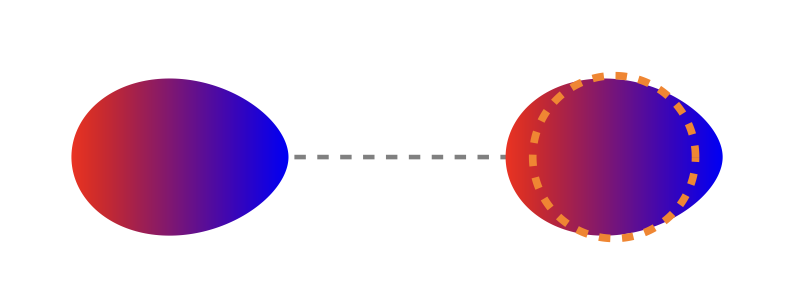
\includegraphics[scale=0.3]{img/0018.2.png}\end{center}
    \item[III]\textbf{瞬时偶极—感应偶极相互作用},又称\textit{London disperson force}:由非极性分子中的瞬时偶极矩,及其诱导的偶极之间的相互作用贡献.%\begin{center}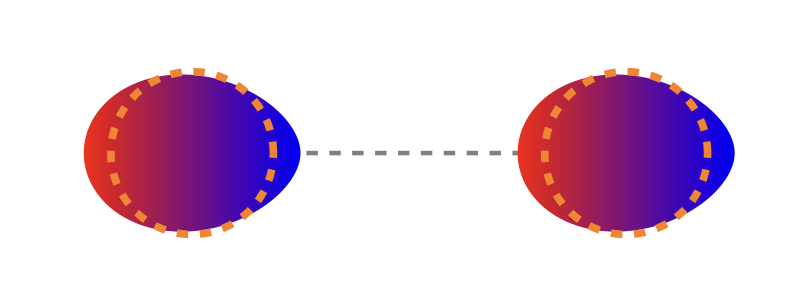
\includegraphics[scale=0.3]{img/0018.3.png}\end{center}
\end{itemize}
这三个相互作用的大小关系大概是$Keesom:Debye:London\approx 100:10:1$,下分别求解这三个相互作用。
\begin{itemize}
    \item[(1)]给定两个偶极矩$\overrightarrow{p_1},\overrightarrow{p_2}$,两者之间的相对矢径为$\overrightarrow{r}$,给出两者相互作用势能$U(\theta_1,\theta_2,\varphi,r)$,$\theta_1,\theta_2,\varphi_1,r$见下图.
    \begin{center}
        \begin{tikzpicture}
            \draw (-6,0) -- (6,0);
            \draw[-{Stealth[length=4mm,width=2mm]}] (-5,-1) -- (-3,1);
            \draw[-{Stealth[length=4mm,width=2mm]}] (2.5,-1)-- (5.5,1);
            \filldraw [black]
            (-5,-1) circle [radius=2pt]
            (-3,1) circle [radius=2pt]
            (2.5,-1) circle [radius=2pt]
            (5.5,1) circle [radius=2pt];
            \draw (-3.7,0) arc [start angle=0, end angle=45, radius=3mm];
            \draw (4.3,0) arc [start angle=0, end angle=33.8, radius=3mm];
            \draw (-3.2,0) node[above] {$\theta_1$};
            \draw (4.8,0) node[above] {$\theta_2$};
            \draw (-4,0) node[above] {$\overrightarrow{p_1}$};
            \draw (4,0) node[above] {$\overrightarrow{p_2}$};
            \draw [<-](2,0) arc (0:300:0.5 and 1);
            \draw (2,1) node[above] {相对转动角$\varphi$};
            \draw (0,0) node[above] {$\overrightarrow{r}$};
        \end{tikzpicture}
    \end{center}
    \item[(2)]现考虑偶极—偶极相互作用,假设电偶极的角分布满足Boltzmann分布,即能量$\varepsilon$出现的概率正比于\ $\exp\left(-\dfrac{\varepsilon}{k_B T}\right)$\ ,且满足$\varepsilon\sim \dfrac{1}{4\pi\varepsilon_0}\dfrac{\overrightarrow{p_1}\cdot\overrightarrow{p_2}}{r^3}\ll k_B T$,给出两个偶极矩之间的平均相互作用势能(保留至最低阶非零项).
    \item[(3)]分子极化率定义为$\alpha=\dfrac{|\overrightarrow{p}_{\mathrm{induced}}|}{|\overrightarrow{E}|}$,即感应偶极矩大小与偶极矩所在点的电场强度大小的比值,偶极矩方向与电场方向相同。现给定$\alpha$,求偶极—感应偶极相互作用势能大小(这里认为$\overrightarrow{p_1}$为源,而$\overrightarrow{p_2}$为感应偶极矩,且其并无自身偶极矩,各角度同上图).
    \item[(4)]接上问,依旧认为电偶极的角分布满足Boltzmann分布,与$\varepsilon\sim \dfrac{1}{4\pi\varepsilon_0}\dfrac{\overrightarrow{p_1}\cdot\overrightarrow{p_2}}{r^3}\ll k_B T$,求其平均偶极—感应偶极相互作用势能大小(保留至最低阶非零项).
\end{itemize}
数学补充:
\begin{equation*}
    \dfrac{\partial }{\partial \beta}\ln \int \exp(\beta x) \mathrm{d}x =\dfrac{\int x \exp(\beta x) \mathrm{d}x}{\int \exp(\beta x) \mathrm{d}x}
\end{equation*}
\end{document} 